\documentclass[10pt]{article}

\usepackage[margin=1in]{geometry}
\usepackage{graphicx}
\usepackage{booktabs}
\usepackage{caption}
\usepackage{xcolor}
\usepackage{amsmath}

\newcommand{\pval}[1]{$p = #1$}

\begin{document}

\section{LLM-as-Judge Evaluation}
\label{sec:llm-judge}

\subsection{Method}
\label{sec:llm-judge-method}

The user study in Section~\ref{sec:results} covers 28 live participants. To test the system at a scale no live study can reach, we also ran an automated evaluation: an LLM judge (GPT-4o, temperature 0) reads two story transcripts and scores them.

The judge is used in two modes. In \textbf{pairwise} mode it reads Story A and Story B side by side and picks a winner per dimension, or calls it a tie. In \textbf{single-story} mode it scores one transcript alone, 0 to 10 per dimension. Every comparison in this section uses both: pairwise for head-to-head verdicts, single-story for the underlying scores those verdicts summarize.

LLM judges are known to favor whichever story happens to be shown first. We control for this directly: every pair is judged twice, once as (A, B) and once as (B, A), and a dimension only gets a winner if both orderings agree once the labels are translated back. If they disagree, the dimension is recorded as a tie. This makes our win counts conservative — a real but small preference is absorbed into ties rather than reported as a win — but it also means a reported win is a robust one, not an artifact of presentation order.

The judge scores stories against a shared rubric, extended for each comparison type. The core 8 dimensions apply everywhere; each comparison type adds a few more.

\begin{table}[htbp]
\centering
\caption{Judge rubric dimensions.}
\label{tab:rubric}
\small
\begin{tabular}{p{3.3cm}p{10.5cm}}
\toprule
Dimension & What it measures \\
\midrule
Plot & Clear beginning/middle/end; reaches the intended beats; no logical holes. \\
Development & Characters and setting are introduced with enough detail to feel real. \\
Language Use & Varied, expressive, in-character language; not bland or repetitive. \\
Interruption Handling & Handles off-topic input gracefully and steers back without derailing or looping. \\
Character Fidelity & Stays in character; doesn't sound like a generic assistant. \\
Narrative Control & Makes steady progress through the beats; doesn't get stuck. \\
Anthropomorphism & Feels like an autonomous character with agency, not a tool serving the user. \\
Overall & Holistic judgment across all of the above. \\
\midrule
\multicolumn{2}{l}{\textit{Added for director vs.\ CoDi:}} \\
Detail \& Thoroughness & Rich description, world-building, thorough scenes. \\
Narrative Polish & Smooth, well-edited prose; natural transitions. \\
Director Decision-Making & How clearly the director's own choices guided the story. \\
\midrule
\multicolumn{2}{l}{\textit{Used instead, for the time-budget ablation (single-story only):}} \\
Descriptiveness & Sensory detail and interiority appropriate to the time budget. \\
Beat Fidelity & Each beat is honored in substance, not just touched on, despite time pressure. \\
Transition Quality & Scene breaks feel motivated, not abrupt or mid-sentence. \\
Three-Act Balance & A recognizable beginning/middle/end survives the compression. \\
Setup/Payoff Preservation & Anything planted earlier is still paid off. \\
Emotional Arc & The emotional register visibly shifts across the story. \\
\bottomrule
\end{tabular}
\end{table}

We ran three separate comparisons:

\begin{itemize}
\item \textbf{Baseline vs.\ director} (Section~\ref{sec:llm-baseline}) — 33 transcript pairs: 10 Olaf story scenarios, each played at three derailment levels (none, medium, complete), plus a 3-scenario Red Riding Hood pilot set at the same three levels.
\item \textbf{Director vs.\ CoDi} (Section~\ref{sec:llm-codi}) — 30 transcript pairs: the same 10 Olaf scenarios x 3 derailment levels, this time against CoDi, an external multi-agent story-generation framework used as a second baseline.
\item \textbf{Time-budget ablation} (Section~\ref{sec:llm-time}) — the time-constrained director run at four fixed budgets (0.5, 2, 5, 10 minutes) against each other and against the unconstrained director, across the same 30 scenarios, scored single-story only (comparing stories of different lengths pairwise is not meaningful).
\end{itemize}

All three use the same underlying transcripts, character prompts, and scenario set as the rest of this thesis — only the evaluator changes, from live participants to an LLM judge.

\subsection{Baseline vs.\ Director}
\label{sec:llm-baseline}

\begin{figure}[htbp]
\centering
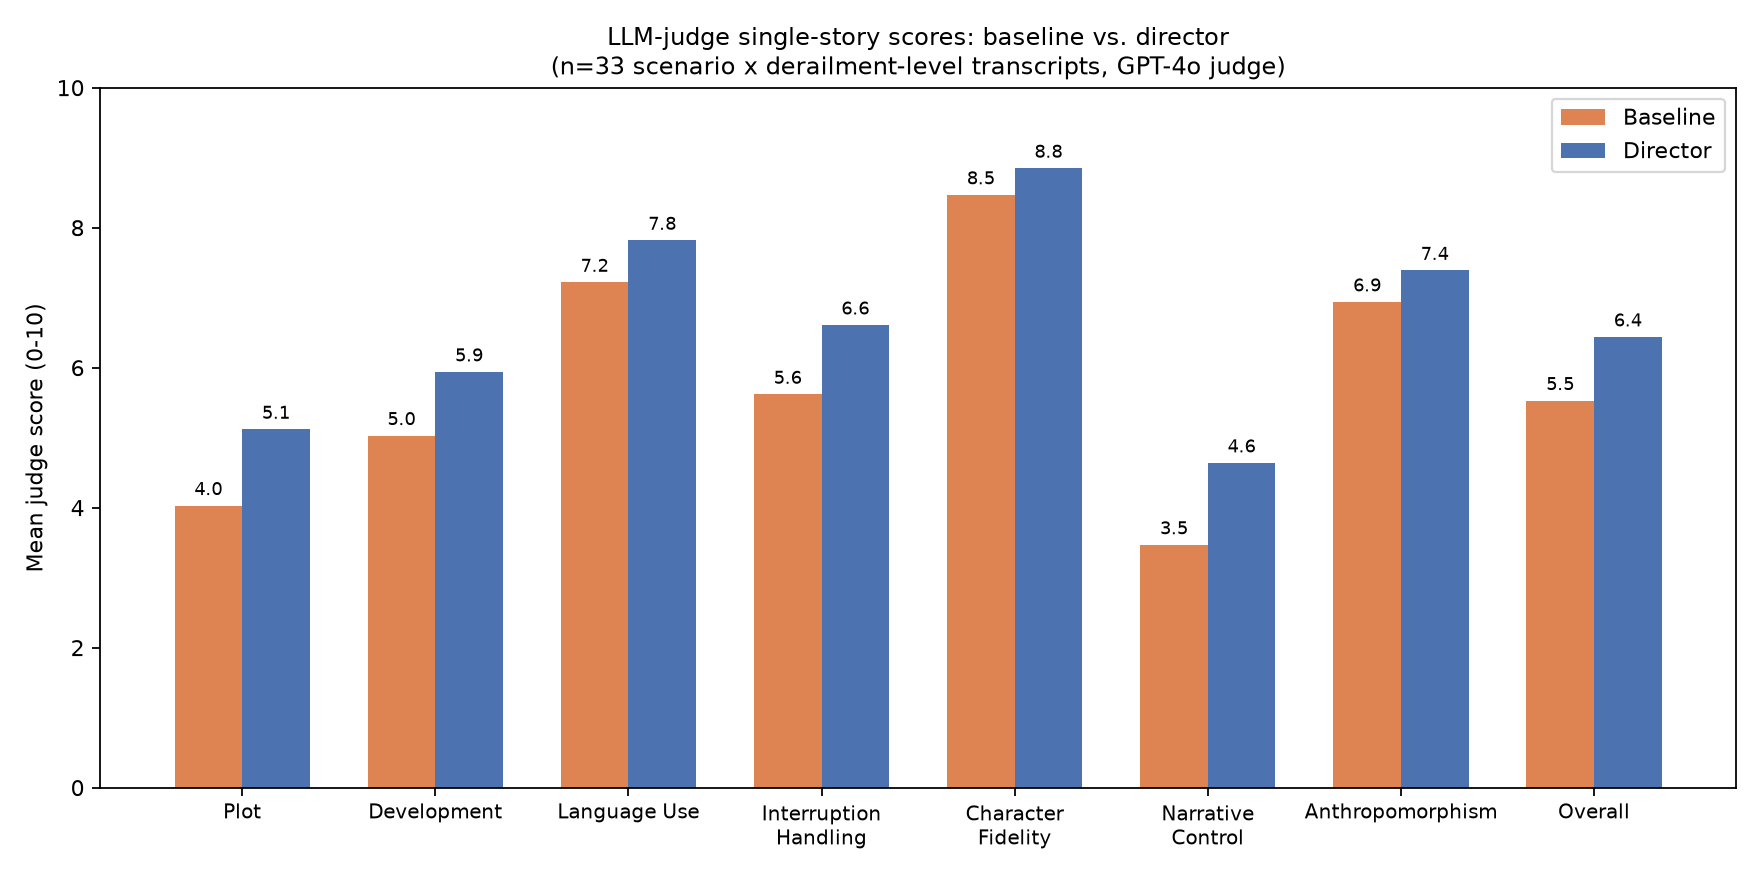
\includegraphics[width=0.95\linewidth]{plots/01_baseline_vs_director_scores_by_metric.png}
\caption{Single-story judge scores, baseline vs.\ director, averaged over all 33 transcript pairs.}
\label{fig:llm-base-metric}
\end{figure}

\begin{table}[htbp]
\centering
\caption{Baseline vs.\ director, mean single-story score per dimension (n=33 pairs).}
\label{tab:llm-base-metric}
\begin{tabular}{lcc}
\toprule
Dimension & Baseline & Director \\
\midrule
Plot                   & 4.03 & 5.12 \\
Development             & 5.03 & 5.94 \\
Language Use            & 7.22 & 7.82 \\
Interruption Handling   & 5.62 & 6.61 \\
Character Fidelity      & 8.47 & 8.85 \\
Narrative Control       & 3.47 & 4.64 \\
Anthropomorphism        & 6.94 & 7.39 \\
Overall                  & 5.53 & 6.44 \\
\bottomrule
\end{tabular}
\end{table}

Director scores higher on every single dimension. The gap is largest on Narrative Control and Plot — exactly where a director layer should help, since its whole job is steering the story toward its beats. Character Fidelity is already high under baseline (8.47) and only edges up slightly (8.85): as in the live study, staying in character is not baseline's weak point.

\begin{figure}[htbp]
\centering
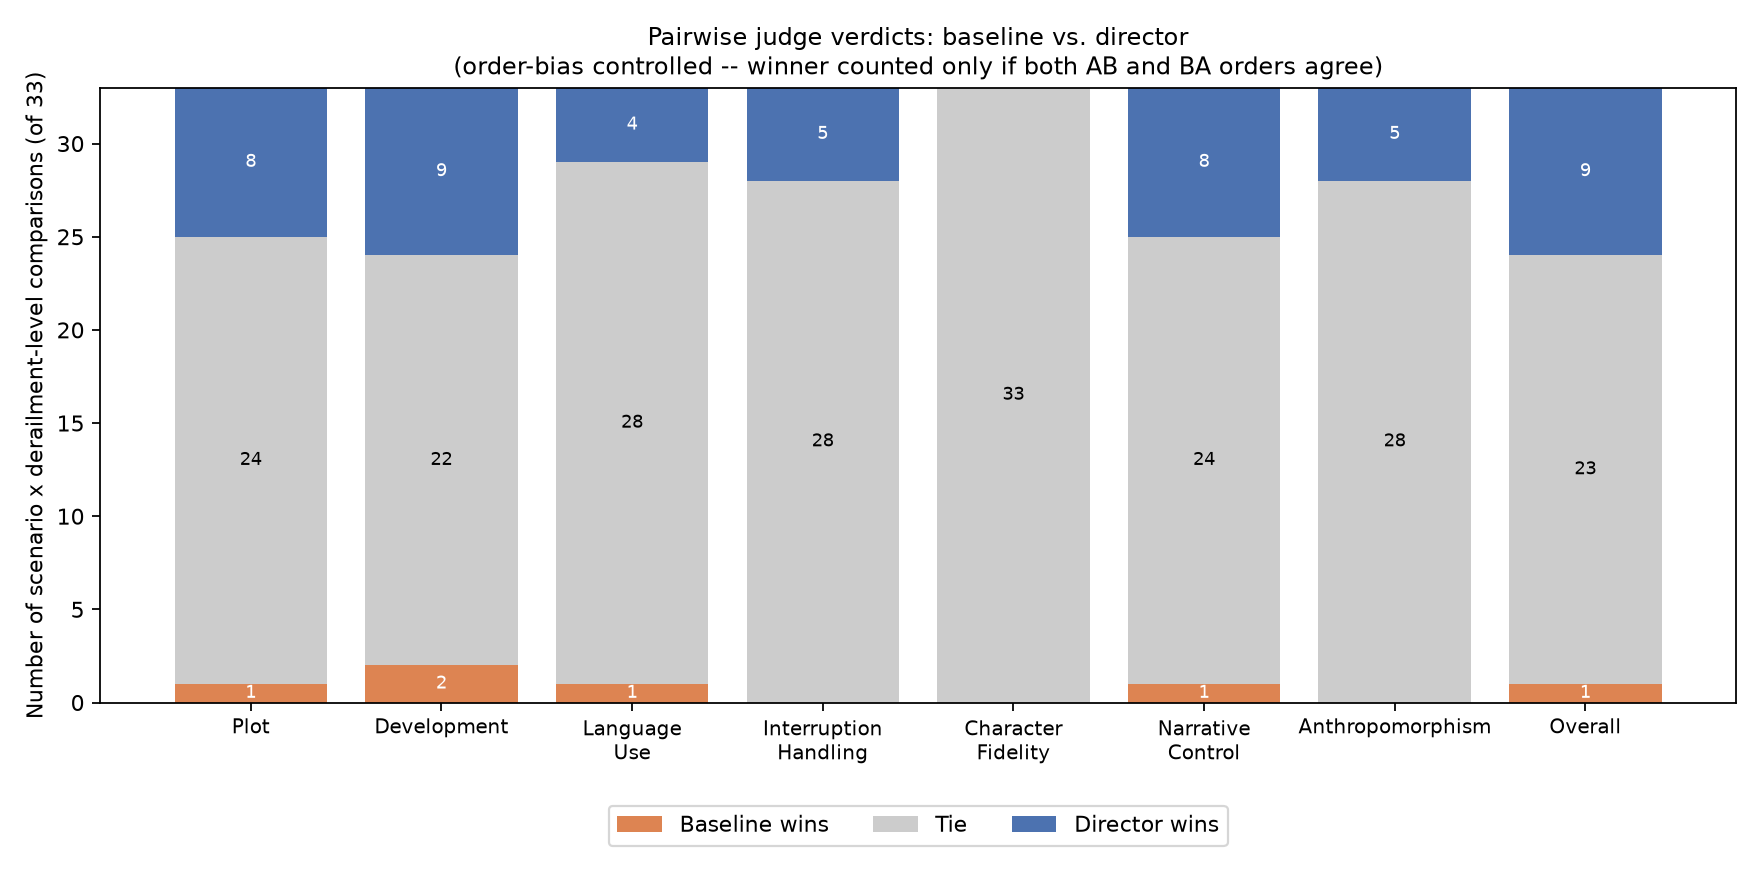
\includegraphics[width=0.95\linewidth]{plots/02_baseline_vs_director_pairwise_wins.png}
\caption{Pairwise verdicts, baseline vs.\ director, order-bias controlled (n=33).}
\label{fig:llm-base-wins}
\end{figure}

The pairwise verdicts (Figure~\ref{fig:llm-base-wins}) tell a stricter version of the same story. Because a win only counts when both presentation orders agree, ties dominate every dimension — but where a winner does emerge, it is almost always director. Baseline wins outright on only 6 of 264 dimension judgments across all 33 pairs; director wins 48. On Character Fidelity, the judge never picks a winner at all (33/33 tied) — full agreement that this dimension is a wash. One assessment, on a scenario with complete derailment, makes the pattern concrete:

\begin{quote}
\small
``Story A struggles with handling interruptions, often getting stuck in the same beat and failing to progress the story effectively. Story B handles interruptions more gracefully by acknowledging them and then redirecting back to the story. This approach keeps the narrative on track and maintains coherence.''
\end{quote}

\begin{figure}[htbp]
\centering
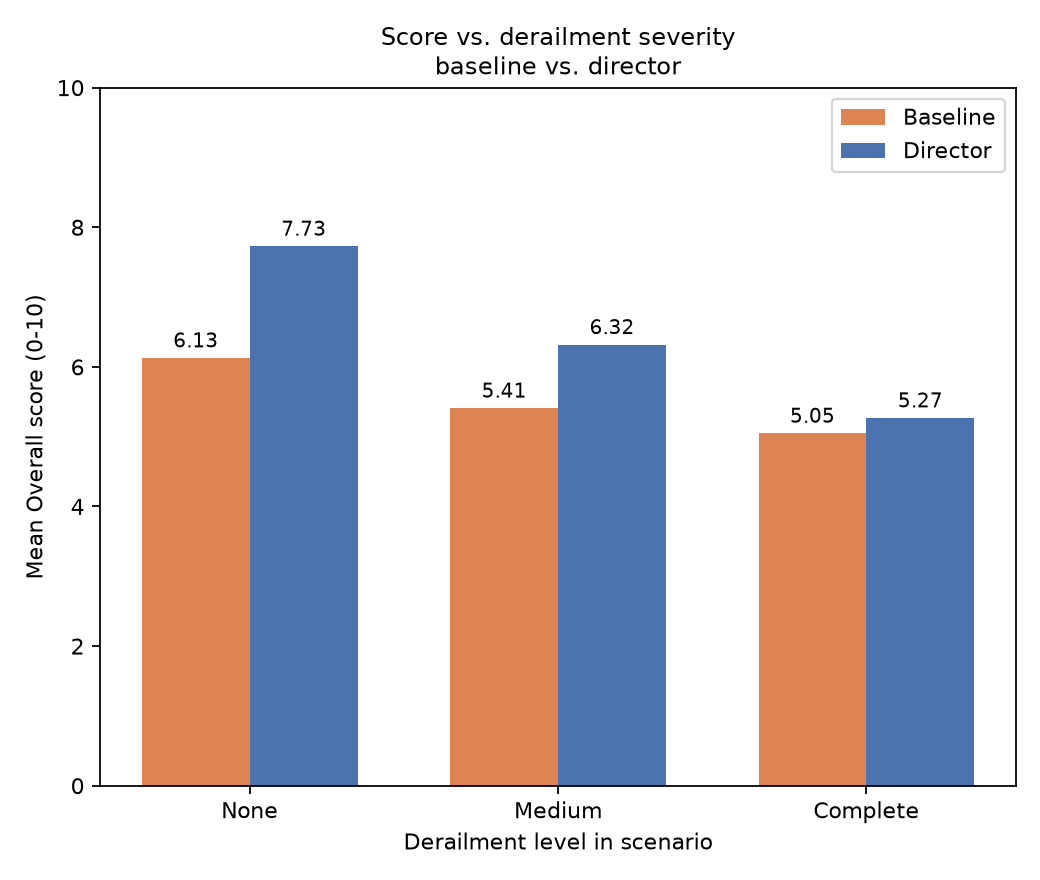
\includegraphics[width=0.6\linewidth]{plots/03_baseline_vs_director_by_derailment_level.png}
\caption{Overall score vs.\ derailment severity, baseline vs.\ director.}
\label{fig:llm-base-derail}
\end{figure}

\begin{table}[htbp]
\centering
\caption{Overall score by derailment level.}
\label{tab:llm-base-derail}
\begin{tabular}{lccc}
\toprule
 & None & Medium & Complete \\
\midrule
Baseline & 6.13 & 5.41 & 5.05 \\
Director & 7.73 & 6.32 & 5.27 \\
\bottomrule
\end{tabular}
\end{table}

Both systems degrade as derailment gets more severe, which is expected — more off-topic pressure is genuinely harder to handle. But director's lead over baseline shrinks as it goes: 1.60 points at no derailment, 0.91 at medium, down to 0.22 at complete. Under the heaviest pressure, the gap nearly closes. This lines up with the automated track's overall picture: director is a clear improvement, but it is not immune to derailment, only more resistant to it.

\subsection{Director vs.\ CoDi}
\label{sec:llm-codi}

CoDi is an external multi-agent story-generation framework, included as a second point of comparison beyond our own baseline. Where the director-vs-baseline comparison isolates the value of adding a director layer at all, this comparison asks a harder question: how does our specific director design compare to another system built for the same job.

\begin{figure}[htbp]
\centering
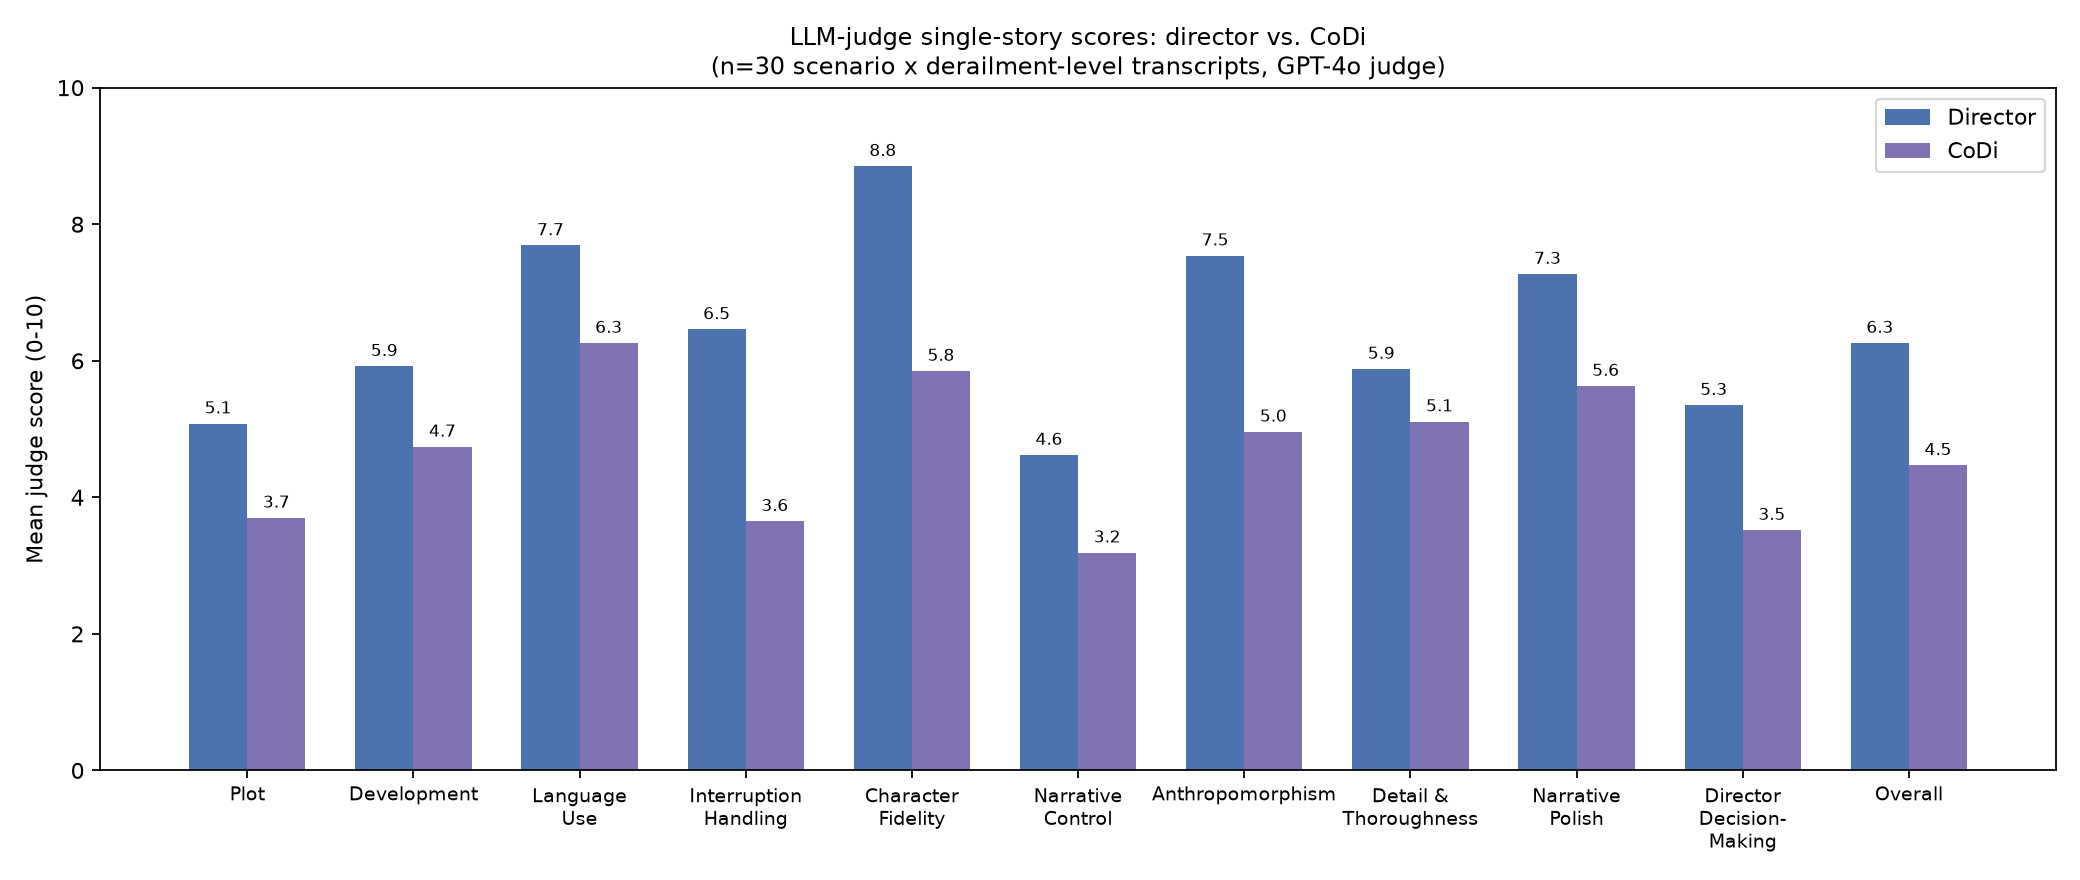
\includegraphics[width=0.95\linewidth]{plots/04_director_vs_codi_scores_by_metric.png}
\caption{Single-story judge scores, director vs.\ CoDi, averaged over 30 transcript pairs.}
\label{fig:llm-codi-metric}
\end{figure}

\begin{table}[htbp]
\centering
\caption{Director vs.\ CoDi, mean single-story score per dimension (n=30 pairs).}
\label{tab:llm-codi-metric}
\begin{tabular}{lcc}
\toprule
Dimension & Director & CoDi \\
\midrule
Plot                       & 5.08 & 3.70 \\
Development                 & 5.92 & 4.74 \\
Language Use                & 7.69 & 6.26 \\
Interruption Handling       & 6.46 & 3.65 \\
Character Fidelity          & 8.85 & 5.85 \\
Narrative Control           & 4.62 & 3.19 \\
Anthropomorphism            & 7.54 & 4.96 \\
Detail \& Thoroughness       & 5.88 & 5.11 \\
Narrative Polish            & 7.27 & 5.63 \\
Director Decision-Making    & 5.35 & 3.52 \\
Overall                      & 6.26 & 4.47 \\
\bottomrule
\end{tabular}
\end{table}

Director scores higher on every dimension here too, including the three added specifically to give CoDi's multi-agent planning a fair shot (Detail \& Thoroughness, Narrative Polish, Director Decision-Making). The margin is largest on Character Fidelity (+3.00) and Interruption Handling (+2.81) — the two dimensions most directly tied to staying in character while being interrupted.

\begin{figure}[htbp]
\centering
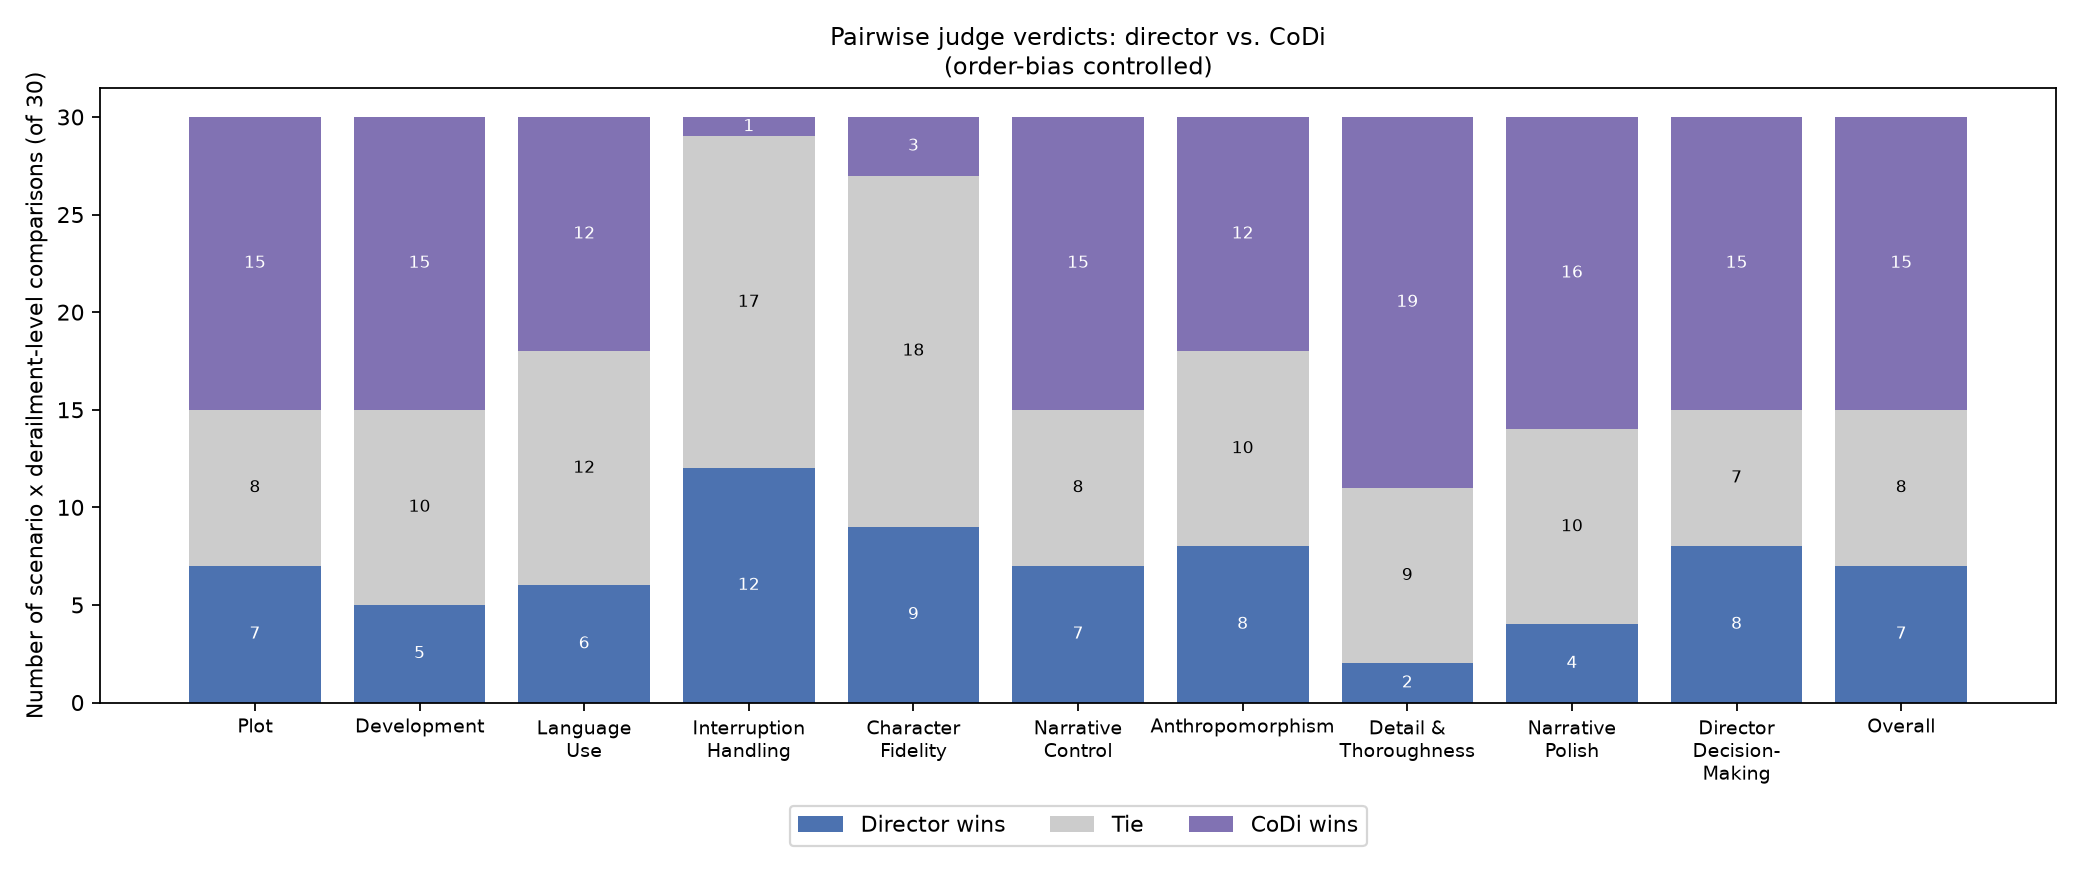
\includegraphics[width=0.95\linewidth]{plots/05_director_vs_codi_pairwise_wins.png}
\caption{Pairwise verdicts, director vs.\ CoDi, order-bias controlled (n=30).}
\label{fig:llm-codi-wins}
\end{figure}

The pairwise verdicts complicate this picture in an interesting way. CoDi wins outright on Plot, Development, Narrative Control, Detail \& Thoroughness, Narrative Polish, and Director Decision-Making — the dimensions about craft and planning. Director wins outright on exactly two: Interruption Handling (12 wins vs.\ CoDi's 1, 17 ties) and Character Fidelity (9 vs.\ 3, 18 ties). One assessment states the trade-off directly:

\begin{quote}
\small
``System A [director] effectively manages interruptions, keeping the narrative on track, albeit at the cost of progression.'' \\
``The narrative includes rich descriptions and thorough scene development, providing a comprehensive and immersive experience'' [System B, CoDi, on Detail \& Thoroughness].
\end{quote}

So the two systems specialize. CoDi, with more planning overhead, produces more detailed, better-plotted prose when left alone. Director is worse at that, but it is built specifically to keep a live, interruptible conversation on track without breaking character — and on exactly that axis, it beats CoDi more decisively than on anything else. Given that interruption handling is the central problem this thesis addresses, this is the more relevant result of the two, even though it is not where director wins the most dimensions.

\subsection{Time-Budget Ablation}
\label{sec:llm-time}

The live user study tests one time budget (5 minutes) against no budget at all. Here we test four fixed budgets — 0.5, 2, 5, and 10 minutes — against each other and against the unconstrained director, all on the same 30 scenarios, using two rule-based structural metrics (no LLM involved) alongside the judge's qualitative score.

\begin{figure}[htbp]
\centering
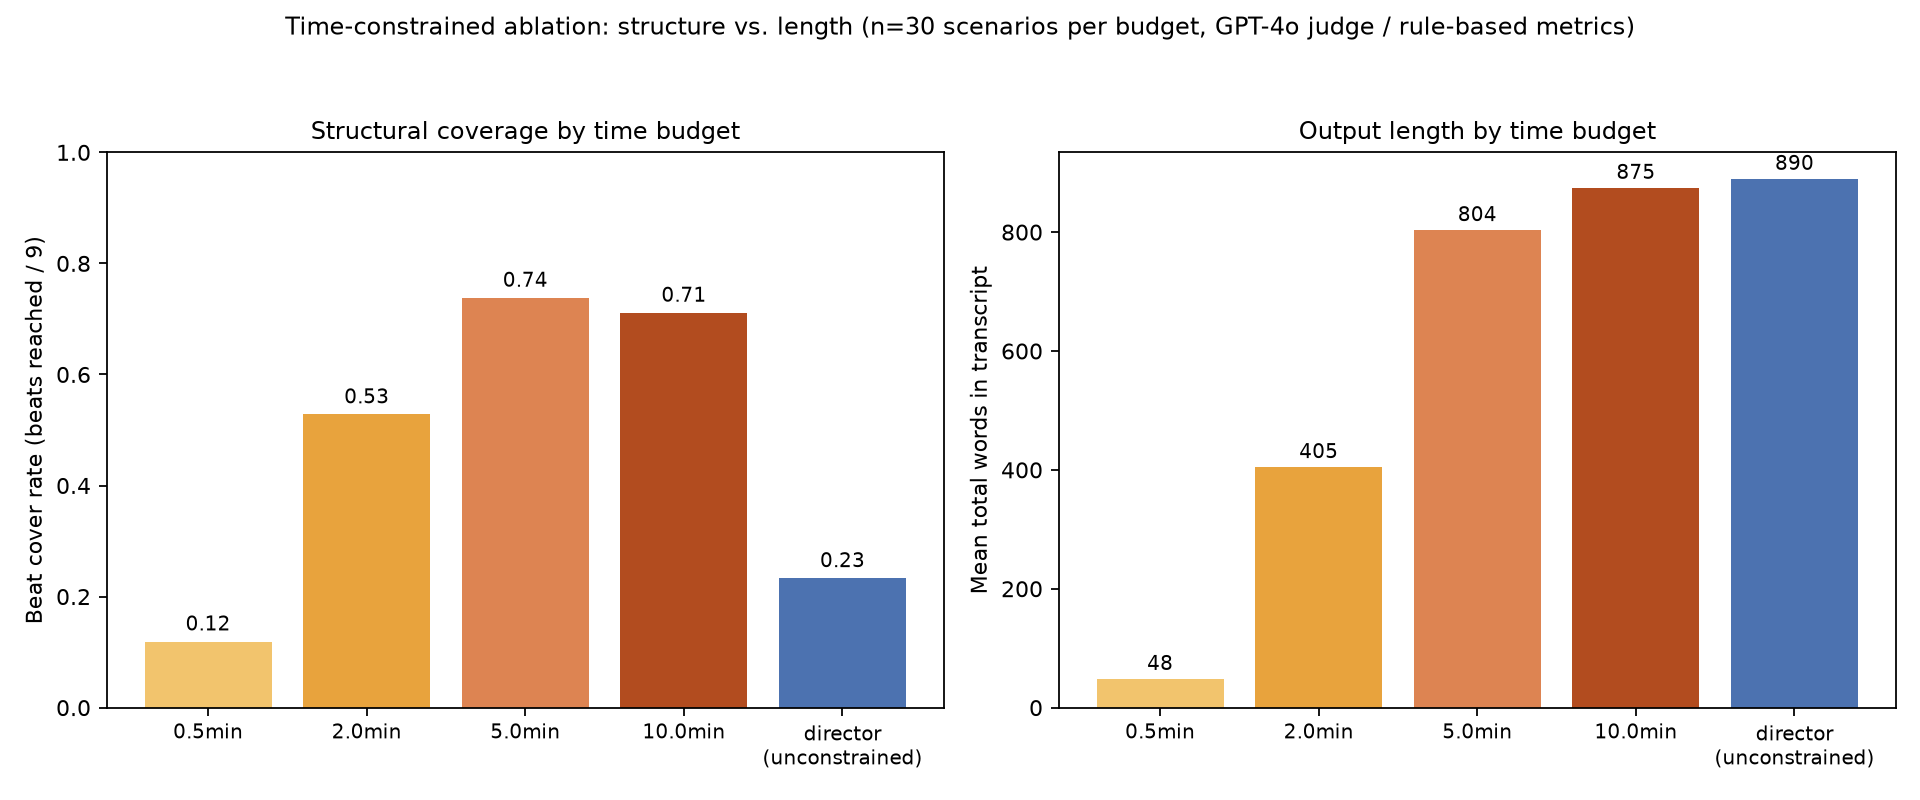
\includegraphics[width=0.95\linewidth]{plots/06_time_constrained_coverage_and_length.png}
\caption{Beat coverage and output length across time budgets (n=30 scenarios per budget).}
\label{fig:llm-time-coverage}
\end{figure}

\begin{table}[htbp]
\centering
\caption{Structural metrics by time budget.}
\label{tab:llm-time-metrics}
\begin{tabular}{lccccc}
\toprule
 & 0.5min & 2.0min & 5.0min & 10.0min & Director (unconstrained) \\
\midrule
Beat cover rate      & 0.12 & 0.53 & 0.74 & 0.71 & 0.23 \\
Total words (mean)   & 48   & 405  & 804  & 875  & 890 \\
Truncated (share)    & 100\% & 100\% & 100\% & 100\% & 100\% \\
\bottomrule
\end{tabular}
\end{table}

Beat coverage rises sharply from 0.5 to 5 minutes, then \emph{plateaus and slightly drops} from 5 to 10 minutes (0.74 to 0.71) — more time past a point does not buy more structure. The unconstrained director is the extreme case: it produces the most words of any condition (890, more even than the 10-minute budget) but covers the fewest beats (0.23) — almost the same wasteful pattern the live study found, where the unconstrained round rarely reached an ending despite generating plenty of text. And every single transcript in this ablation, at every budget including 10 minutes, is flagged as truncated: none of them cleanly complete their final beat. A time budget changes how much of the story gets told, not whether it finishes cleanly.

\begin{figure}[htbp]
\centering
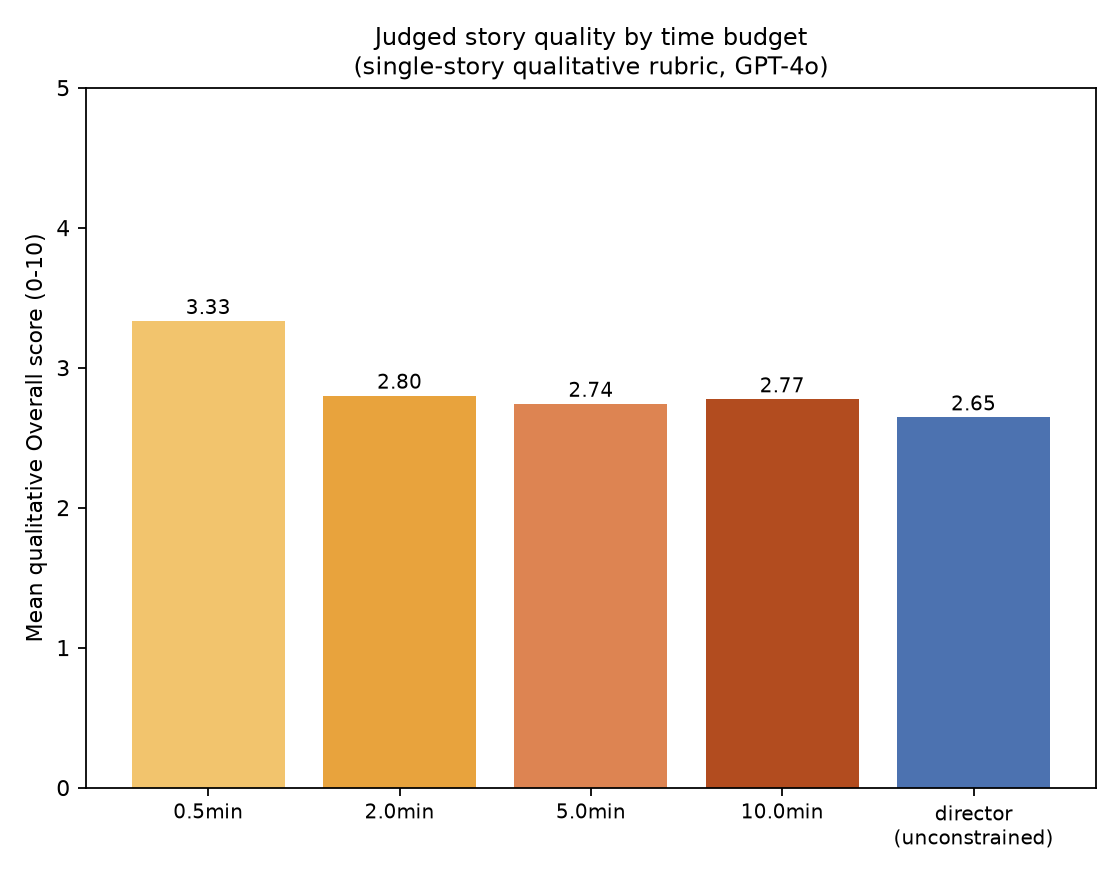
\includegraphics[width=0.65\linewidth]{plots/07_time_constrained_qualitative_overall.png}
\caption{Judged story quality (single-story Overall) by time budget.}
\label{fig:llm-time-qual}
\end{figure}

The judged quality score (Figure~\ref{fig:llm-time-qual}) runs the other way: it is \emph{highest} at 0.5 minutes (3.33) and lowest for the unconstrained director (2.65), with 2--10 minutes clustered in between. This looks backwards until read alongside Table~\ref{tab:llm-time-metrics}: a 0.5-minute story is a single short scene, with almost nothing in it to go wrong — no time to lose the thread, repeat itself, or mishandle an interruption. The judge was explicitly instructed not to penalize a short story for being short, and a near-empty story is easy to rate as clean. Longer, more structurally complete stories have more surface area for judged flaws, even though they objectively cover more of the plot. We read this as a limitation of a single-story quality score under a time constraint, not as evidence that shorter is actually better — the beat-coverage numbers in Table~\ref{tab:llm-time-metrics} are the more trustworthy measure of what these budgets actually accomplish.

Finally, embedding-based cosine similarity between transcripts at different budgets (Table~\ref{tab:llm-time-sim}) shows budgets close in length stay close in content (5 vs.\ 10 minutes: 0.91) while the 0.5-minute condition diverges from everything else (0.66--0.69) — consistent with it being a different, much shorter story rather than a compressed version of the same one.

\begin{table}[htbp]
\centering
\caption{Pairwise cosine similarity between transcripts at different time budgets, averaged across scenarios.}
\label{tab:llm-time-sim}
\begin{tabular}{lccccc}
\toprule
 & 0.5min & 2.0min & 5.0min & 10.0min & Director \\
\midrule
0.5min    & 1.00 & 0.76 & 0.68 & 0.69 & 0.67 \\
2.0min    & 0.76 & 1.00 & 0.88 & 0.86 & 0.84 \\
5.0min    & 0.68 & 0.88 & 1.00 & 0.91 & 0.88 \\
10.0min   & 0.69 & 0.86 & 0.91 & 1.00 & 0.89 \\
Director  & 0.67 & 0.84 & 0.88 & 0.89 & 1.00 \\
\bottomrule
\end{tabular}
\end{table}

\subsection{Summary}
\label{sec:llm-summary}

\begin{itemize}
\item Director beats baseline on every judged dimension, with the clearest, most consistent margins on Narrative Control and Plot — the director layer does what it is designed to do.
\item Director's advantage over baseline shrinks as derailment gets more severe (1.60 points at no derailment, down to 0.22 under complete derailment) — confirmation, from an independent evaluator, that heavy derailment is genuinely hard, not that the director stops helping.
\item Against CoDi, the two systems trade off: CoDi produces more detailed, better-plotted prose; director wins decisively on Interruption Handling and Character Fidelity — the two dimensions this thesis is actually about.
\item More time budget does not mean the story finishes: every time-constrained transcript in the ablation, at every budget tested, is truncated before a clean ending, and coverage plateaus past 5 minutes.
\item The unconstrained director is the least structurally complete condition of all despite producing the most text — the same pattern the live user study found, now confirmed on 30 additional scenarios by an independent judge.
\end{itemize}

\end{document}
